\documentclass[10pt,letterpaper]{article}
\usepackage[utf8]{inputenc}
\usepackage{amsmath}
\usepackage{amsfonts}
\usepackage{amssymb}
\usepackage{hyperref}
\usepackage{makeidx}
\usepackage{graphicx}
\usepackage{float}
\usepackage{svg}
\usepackage{subcaption}
\usepackage{fancyhdr}
\usepackage{float}
\usepackage{tikz}
\usepackage{nth}
\usepackage{multicol}
\usepackage{siunitx}
\usepackage[default,scale=1.0]{opensans}
\usepackage[margin=1in]{geometry}

%% Preamble
% Custom commands
\newcommand{\ts}{\textsubscript}

% Hyper ref
\hypersetup{
	colorlinks=true,
	citecolor=black,
	linkcolor=black,
	filecolor=black,
	urlcolor=blue,
	pdftitle={APSC 210 Report - Muchen He},
	bookmarks=true
}
\urlstyle{same}

% Page semantics
\pagestyle{fancy}
\fancyhead[L]{\slshape\MakeUppercase{APSC 210}}
\fancyhead[R]{\slshape Muchen He}
\fancyfoot{}
\fancyfoot[C]{\thepage}

\parindent 0ex

% Meta
\author{Muchen He}
\title{APSC 210 Work Term Report}
\begin{document}
\begin{titlepage}
	\begin{center}
		\vspace*{3in}
		\line(1, 0){400}\\
		\Huge{\textbf{Game Dev @ BioWare}}\\[0.2cm]
		\large{\textbf{Career Development Report (Work Term 2)}}\\[1cm]
		\Large{\textbf{APSC 210}}\\
		\textbf{University of British Columbia}\\
		\line(1, 0){400}\\
		\vfill
		\Large{Muchen He}\\
		\large{Associate Developer, BioWare Edmonton}\\
		44638154\\

		\today \\
	\end{center}
\end{titlepage}

% Table of contents
\setcounter{secnumdepth}{3}
\tableofcontents
\thispagestyle{empty}
\clearpage

% list of tables and figures
\thispagestyle{empty}
\listoffigures
\listoftables
\newpage

\setcounter{page}{1}
\setcounter{section}{-1}

% Starting of report content
\section{Introduction}\label{introduction}

\subsection{Outline}\label{introduction-outline}

This report serves to probe the progression of career development. This report is written with intent to achieve helping us gauge our current desired career path by reviewing the skills obtained throughout the work term, as well as future desired skills that would be necessary for future careers. \\
\\
The report is broken down into four parts to help us understand what is it we need to proceed in our career development: industry in current work term, current skills being obtained, desired future industry, and transferable skills that might aid us reaching there.\\
\\
The report will also briefly describe the company and the industry it takes position in. The studio that I work for is BioWare, which is a subsidiary of a larger publisher, Electronic Arts (EA).

\subsection{Scope}\label{introduction-scope}

The scope of report consists of analysis of skills and duty pertained to me and future desired skills. The report will not include details about the game, engine, or other technology used during the work term that helped me obtaining skills or reach my objectives.

\subsection{Industry}\label{introduction-industry}

EA or BioWare, like many other studios or publishers exist in the market right now  falls into the consumer entertainment industry. The products produced is associated with Microsoft and Sony as they develop the hardware the games will run on. Future industries I wish to work in consist of electronics development or robotics and control systems.\\
\\
\textit{Work Term Industry} (section \ref{work-term-industry}) provides insight the industry with which we are currently working and competing in. This section outlines the company's position and its competitions in the gaming and or online entertainment and content delivery industry.

\subsection{Company}\label{introduction-company}

BioWare is a game development studio founded in 1995 by three medical doctors in Edmonton, Alberta\cite{bioware-wiki}. Since the establishment, BioWare has developed numerous titles including the Mass Effect and Dragon Age franchise as well as the massive multiplier online (MMO) game Star Wars: The Old Republic. BioWare is currently developing Anthem, the upcoming game set to release in Feburary, 2019.\\
\\
The company is now a division of EA, which is an American video game publishing company. This allows for cross-studio sharing of technology. Such as using the Frostbite engine (game engine developed by another EA studio, DICE, in Sweden) instead of using the in-house engine BioWare developed \cite{frostbite-wiki}\cite{eadice-wiki}. In 2018, BioWare went through rebranding that replaced the logos (figure \ref{fig:biowarelogos}).\cite{bioware-wiki}\\
\\
\begin{figure}[H]
	\centering
	\begin{subfigure}[c]{0.3\textwidth}
		\centering
		
\includegraphics[width=0.7\textwidth]{assets/logo1995}
		\caption{BioWare logo in 1995}
	\end{subfigure}
	~
	\begin{subfigure}[c]{0.3\textwidth}
		\centering
		
\includegraphics[width=0.7\textwidth]{assets/logo2005}
		\caption{BioWare logo prior to rebranding}
	\end{subfigure}
	~
	\begin{subfigure}[c]{0.3\textwidth}
		\centering
		
\includegraphics[width=0.7\textwidth]{assets/logo2018}
		\caption{BioWare logo in 2018}
	\end{subfigure}
	\caption{BioWare logos}
	\label{fig:biowarelogos}
\end{figure}


There is a pipeline of games the studio outputs, the latest one being Anthem, showcased at the Electronic Entertainment Expo (E3) in 2017 and 2018. The game so far has won many E3 awards.\\
\\
To date, there are 800 active employees working at BioWare ranging from artists to programmers. My position is an associate developer on the UI/UX team for the game Anthem. Mostly developing engine tools, and elements the scriptwriters and artists can then use to add feature into the game. \\

\clearpage
\section{Work Term Industry}\label{work-term-industry}

BioWare is computer software company that develops video games for PCs, XBOX, and PlayStation. Thus we fall under \textit{Services - Computer Programming / Software} industry.\\
\\
We will also examine the video game industry in depth because of its relevance and size. \\

\subsection{Industry History}

The software industry primary focuses on developing computer programs as service (SaaS) or product that started in the 1950s. Recently, open source solutions and internet of things (IoT) are popular.\cite{software-industry}\\
\\
The history of video game industry started in the 1970s when computers are powerful enough to run games even though videos exisited since the 40s. Recently, the video game industry has expanded to many platforms including social media, mobile, argumented reality (AR) and virtual reality (VR).\cite{video-game-industry-wiki}\cite{video-game-industry-stats}\\

\subsection{Economic Status}

The video game industry economic status is growing as 

Earlier games in the industry are generally cheap inexpensive to make because of small teams and low demand for quality from the consumers. In recent decades however, large budget games (A.K.A AAA or Triple A games) consists of large development teams and usually takes  a year to three yeear to develop a single game. This is due to increased technological complexity.\cite{cost-game}\\
\\
In 2017, the video game industry was valued at 17.68 billion USD. \cite{video-game-industry-stats}.\\
\\
One competitor in the industry, Rockstar, and their most recent products Grand Theft Auto V (GTA 5) has become the most profitable product in the industry \cite{IGN-gta5}. With a total revenue of \$6 billion, it has made "more money than any film, book, or game".\\
\\
EA's earnings is as show below (figure \ref{fig:ea-revenue})\cite{ea-earnings}. As shown, there is an increasing amount of income from ``Live Serivces''. This includes the after-sale content such as downloadable contents (DLCs) and micro-transactions (MTX) within the published games. Due to its financial appeal, Anthem will follow the same \textit{live services} model. The game will feature purchaseable cosmetic items  and will not have ``lootboxes'' (more details in economic factors section).\\

\begin{figure}[H]
	\centering
	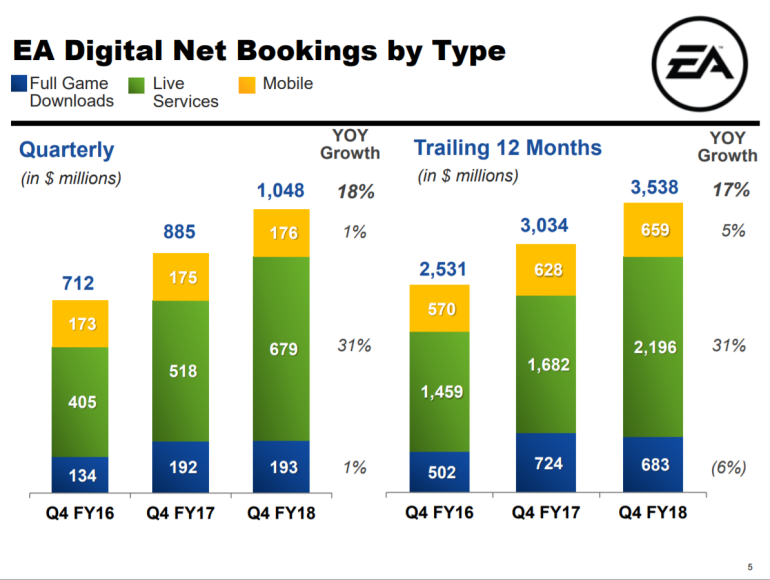
\includegraphics[width=0.6\textwidth]{assets/ea-revenue}
	\caption{EA Earnings by Type}
	\label{fig:ea-revenue}
\end{figure}

\subsection{Geographics \& Concentrations}

The software industry is global. Industry leaders are based in USA. Because one can contribute to software from any computer, there is a large amount of freelancers or open-source contributers that can work from around the world.\\
\\
The video game industry also applies worldwide. The USA is one of the largest producer of video games, most companies and publishers including Electronic Arts, Blizzard - Activision, and Valve (they own the world's largest online video game distribution platform - Steam \cite{steam}).\\
\\
The largest market is China, with MMO games on PC being the largest category \cite{video-game-china}\cite{big-game-china}.

\subsection{Opportunities for Engineers}

For the video game industry, even though the products are viewed as entertainment or arts by the public, there are still many critical roles for engineers. According to Carlos Guerrero, a senior producer at EA, who had worked on games including World of Warcraft (WoW) and Overwatch, there are many technologies that goes into a game that need to be developed and maintained.\\
\\
The following chart depicts various roles that goes into making a game (figure \ref{fig:video-game-as-career}). In fact, the engineers make up a critical part: from video game engine development to online system infrastructure.\\

\begin{figure}[H]
	\centering
	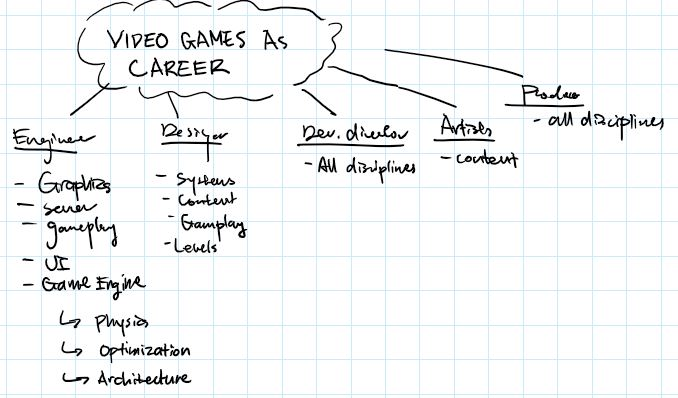
\includegraphics[width=0.6\textwidth]{assets/video-games-career-roles}
	\caption{Video game as career}
	\label{fig:video-game-as-career}
\end{figure}

\subsection{Employers in the Industry}

For computer programming / software industry, the most notable industries include Microsoft, SAP, and ADP. Google and Amazon are also in the industry. Google is advertisement company with its parent company Alphabet owning several subsidiaries in AI research. Likewise, Amazon world's largest cloud computing service Amazon Web Services (AWS).\\
\\
In the scope of the video game industry, EA is one of the biggest publisher in North America which owns subsidiaries including BioWare and DICE.\\
\\
Another large video game publisher is from the giant Tencent, a Chinese internet company. They own Riot, a studio that developed League of Legends (LoL) which has 27 million players daily and an E-sports scene with over 11 million viewership.\cite{lol-wiki}\\

\subsection{Economic Factors}

% TODO:

\begin{center}
	This section intentionally left blank (not applicable).
\end{center}

% The computer programming / software industry has been in high demand for decades. It has evolved 

% The video game industry has also been more relevant than ever. The increase in mobile gaming market and e-sports has 

\subsection{Political Factors}

\begin{center}
	This section intentionally left blank (not applicable).
\end{center}

% - Video game addiction in Asian countries
% - Video game esports influence in SKorea

\clearpage
\section{Obtained Skills}\label{obtained-skills}

% BEGIN of unorganized
This section provides an overview of my technical and non-technical skills gained at BioWare over the course of the work term. \\
\\
Social skills:
- Asking for help from anyone in the office
- Participating in design review

% END of unorganized

\subsection{Technical Skills}

Being in a technical co-op position, the primary skills are comprised of technical skills in software development. The technical skills can be broken down into: fundamental and development workflow skills, programming skills,, and skills invoving specific toolsets.\\

\subsubsection{Fundamental \& Development Skills}

The first category of skills involves fundamentally useful abilities in a development studio.\\
\\
To succeed in this position, one should be proficient in understanding and using version control solutions such as Git (most common) or Perforce (used in enterprise such as Google and EA). Version control is especially important as there are tens or hundreds of developers working on the same project or codebase. It is not uncommon that multiple files undergo ``conflict'' as the same file could be worked on by multiple developers. Therefore explicit version tracking and tools are vital to the workflow.\\
\begin{quote}
	\textit{
It is worth noting that since everyone is working off of the same depot that contains the source code and game data, if one were to break the build, everyone would be affected resulting in many work hours lost.
	}
\end{quote}

One should also be comfortable working with packages and modules (along with its associated package managers) since this makes the project more modular and encourages code reuse (for other licensees). Because of the modularity, one must make no assumptions about how future developers will use this code. Thus, it is important to test extensively, check errors, validate interfaces, and cover edge cases.\\
\\
Moreover, familiarity with agile methodologies is useful in software development environment. Specific actions include code review, time management, and task management with cards (known as ``JIRA'' for EA internals). Each card contains a specific task and is assigned to each person. The card is placed in the person's backlog, and is moved once the task on the card is done.\\
\begin{figure}[H]
	\centering
	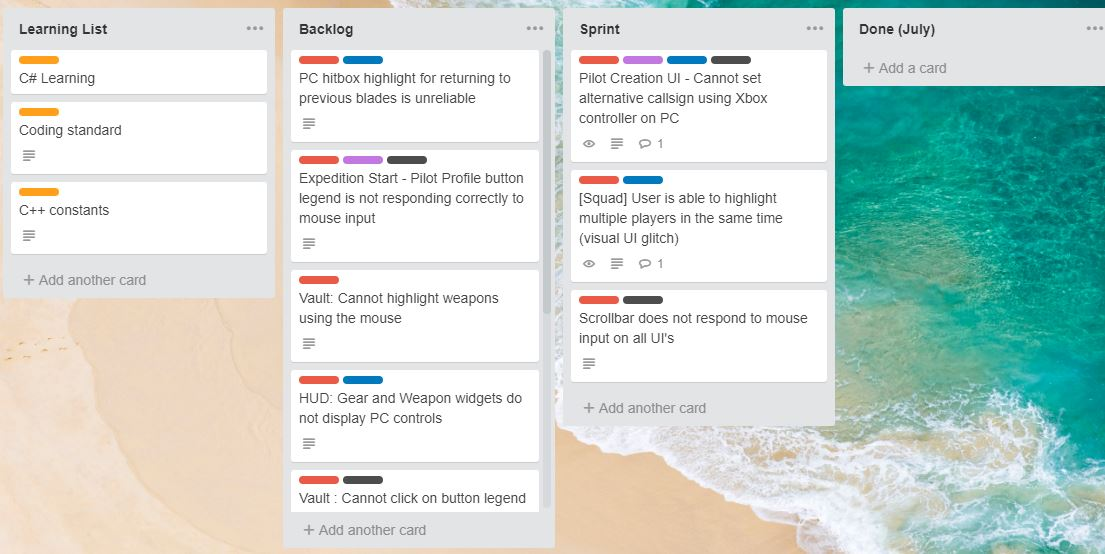
\includegraphics[width=0.75\textwidth]{assets/cards}
	\caption{Cards used in agile methodologies here is depitcted in the app, Trello}
	\label{fig:trello-cards}
\end{figure}
Lastly, contributing to technical documentation such as the development wiki (known as ``confluence'' internally). This can also be considered as a non-technical skill because it overlaps heavily with technical communications, a critical skill required in \textit{any} industry.\\

\subsubsection{Programming Skills}

To success in the video game industry or computer programming industry with heavy enphasis on graphics and physics engines (used ubiquitously in video game production), one should be familiar with C++ the programming language. All AAA video games released in the recent decades are all programmed in C++ or made from game engines made in C++.\\
\\
Of course, knowledge of any progamming language including C or Python helps too as they are useful in specific situtations (and they're used widely in other fields of computer programming: Python is a ``must-have" for AI or machine learning development).\\
\\
At my position at EA, C++ is the logic behind everything in the game. C\# is another programming language that is used widely in UI; it is also the most popular language in amateur game makers as it is used in the free game engine, Unity. We write in C\# for the tools and editors the artists and designers use to make other game content, but ultimately they are ``compiled" into C++. Finally, we write Python scripts to modify game content and assets in bulk.\\
\\
In addition to the specific programming languages, it is also nice to be familair with software concepts such as object oriented programming (OOP), UI/UX design patterns, multithreading to separte rendering and simulation, etc. More details will be in the next report (technial report for APSC 310).\\
\\
Debugging skills and techniques are equally important. The most important skill is to create a conceptual map in mind of where the problem lies, how much or where it is affecting, and where it is coming from by eliminating possibilities. Other techniques include attaching IDE to processes and threads, setting breakpoints and analysing variables in the debugger.\\
\\
Lastly, though it is obvious, it is important to keep in mind that future developers will likely see and use code we write. Writing code that complies with the coding standard, in terms of style of syntax and adding code comments and tags is beneficial.

\subsubsection{Specific Toolset Skills}

These specific toolset skills overlaps with technical skills. But skills involving specific toolsets emphasis on the learning skills. If one can learn, adapt, and use tool given in the development environment, it is and an indication of fast learner.\\
\\
In the current industry of my position, it's useful to understand (at least in context) of what the program or tool is doing under the hood.\\
\\
For instance, the developers use an engine editor called \textit{FrostEd} to make games using the \textit{Frostbite} engine. The editor is a propriatery and private software not distributed to the public, only to EA licensees (game studios). Thus, it is important to learn how to use the editor independently as there lacks online resources, which contributes to enhancing independent learning skills.\\
\\
\textit{FrostEd} is a visual script editor and outputs game assets and schematics used to put together the game. As such, each asset contains references to data, logic, entities, and more. Understanding what was going on underneth these files has helped me greatly in understanding how the editor serializes the assets, and helped me working with the tool and more intuitive in debugging.\\
\\
Perforce, the version control software as mentioned before is another case of skills in specific tools. This is because other companies may employ different version control software such as \texttt{git}.\\

\subsection{Non-Technical Skills}

The most important non-technical skill is learning independently as supervisors or team leads might not always have time to provide all details at all times. Especially if they're often busy.\\
\\
One should always first read through the documentation. Often times, this action is often informally abbreviated as ``RTFM'' which stands for ``Read The F-ing Manual!''. It is also useful to build a mental map or a physcial map of how things fit together.\\
\\
One should use critical thinking using first-principles to sovle problems. Which implies only thinking about what is absolutely true, then progress to what could have happened, then verify the hypothesis and repeat.\\
\\
One important skill that does not get emphasised enough (because of its simplicity) is knowing how to Google (or whichever search engine one prefers). Knowing how to find resources and information online efficiently and accurately saves times can greatly accelerate the learning process.\\
\\
Lastly, it is critical to be mentally healthy during work. Know when to take breaks and relief any frustration that arises during work. Induced frustration and stress often leads to decrease in productivity and cognitive functions.\\
\\
\clearpage
\section{Desired Future Industry}\label{desired-future-industry}

This section outlines my desired future industry to expand my career as well as details about the industry. First I will explore the possible desired industries I want to work at for future work terms.

\subsection{Choosing Desired Industry}

This sub-section intends to provide personal reflection on possible industries in my career progression.\\

\textbf{Depth}\\
I have two choices in mind. The first is software development or computer programming industry. This encourages depth as I already have a few work-terms worth of experiences. Choosing said industry also implies more work on in the UI/UX or app development (relatively front end and higher level) for its high demand. It could be a viable option that consolidates existing technical skills.\\
\\
Possible specific industries include software development (for companies such as Microsoft, Amazon, and start-ups) and video game industry (such as coming back to Electronic Arts or explore other game publishers).\\
\\
The benefit of choosing software industry is that I already possess many skills required to success in this industry. Thus, future job applications are more easier and more fitting. Allowing easier integration and on-boarding into teams of future opportunities.\\
\\
The trade off being that my existing skills in this specific area, which consist of programming in C++, UI/UX and app development, will snowball. As a result, it will be more likely that my future positions be software developer. The career inertia could potentially make it more difficult to enter into  other industries in case of career change.\\
\\
\textbf{Breadth}\\
The second option is to explore industries that differs from pure high-level software development. Industries that could potentially be more related to the my study in electrical engineering. Such as to apply knowledge practiced in courses such as operating and designing electronics or PCBs, mechanical components, apply theories such as controls theory in hardware projects or robotics. The intent would be to try other tasks to expand my set of skills into positions of different industries.\\
\\
Possible industries include electronic and hardware R\&D or design and manufacturing. There are serveral companies that fall under this industry: Intel and Altera for hardware development such as field programmable gate array (FPGA) which are technlogies explored in CPEN courses. Tesla for electric and battery engineering. DJI for drone and robotic applications.\\
\\
The benefit of this route is that to experience new positions, gain insight and additional interests. By expanding skill set, my technical experience is not fixated on software development.\\
\\
For the scope of this report, I will explore the latter industry for a mix of both hardware and low level software/firmware. This falls under the sector outlined on the Co-op handboox\cite{coop-handbook} manufacturing and services sectors; namely ``Computer/Electrical/Electronic Machinary/Equipment" and ``Computer Related Services/Hardware".\\
\\
\subsection{Industry History}

\subsection{Economic Status}
\subsection{Geographics \& Concentrations}
\subsection{Opportunities for Engineers}
\subsection{Employers in the Industry}
\subsection{Economic Factors}
\subsection{Political Factors}

\clearpage
\section{Technical \& Transferable Skills for Senior Work Terms}\label{transferable-skills}

% Unorganized
% Technical communication skills
% - Documentation contribution
% - Coding standard

% Learning Skills
% - Asking for help
% - Knowing how to get help
% -

% Social skills
% - Small talks

This contains the researched required advanced skill for the industry we looked up from talentegg.ca or engineerscareers.ca

\subsection{Self-Marketable Skills Required to Succeed}
\subsubsection{Technical}

\subsubsection{Non-Technical}

\subsection{Plan to Obtain}

\subsubsection{Work Terms}
- reinforce the skills within current workterms that align to those for the future work terms

\subsubsection{In School}
- design teams
- design courses

\subsubsection{Personal Development}
- personal projects
- learn from online courses
- hackathons

\clearpage
\section*{Conclusion}\label{conclusion}
\addcontentsline{toc}{section}{Conclusion}

\clearpage
\begin{thebibliography}{}
	% Bibliography
	
	\bibitem{IGN-gta5}
	Arif, S. (2018, April 9). GTA 5 Has Made More Money Than Any Film, Book, or Game, Says Analyst. Retrieved May 10, 2018, from http://ca.ign.com/articles/2018/04/09/gta-5-has-made-more-money-than-any-film-book-or-game-says-analyst

	\bibitem{bioware}
	BioWare | Rich Stories, Unforgettable Characters, And Vast Worlds. (2018). Retrieved May 23, 2018, from http://www.bioware.com/en/

	\bibitem{bioware-wiki}
	BioWare. (2018, May 23). Retrieved May 23, 2018, from https://en.wikipedia.org/wiki/BioWare

	\bibitem{frostbite-wiki}
	Frostbite (game engine). (2018). Retrieved June 27, 2018, from https://en.wikipedia.org/wiki/Frostbite\_(game\_engine)

	\bibitem{eadice-wiki}
	EA DICE. (2018). Retrieved June 27, 2018, from https://en.wikipedia.org/wiki/EA\_DICE

	\bibitem{ea-earnings}
	EA. (Jan 30, 2018). Electronic Arts Reports Q3 FY18 Financial Results. Retrieved July 5, 2018, from http://news.ea.com/press-release/company-news/electronic-arts-reports-q3-fy18-financial-results

	\bibitem{lol-wiki}
	League of Legends. (2018). Retrieved July 3, 2018, from https://en.wikipedia.org/wiki/League\_of\_Legends.

	\bibitem{bioware-wiki-list}
	List of BioWare video games. (2018, May 22). Retrieved May 23, 2018, from https://en.wikipedia.org/wiki/List\_of\_BioWare\_video\_games

	\bibitem{software-industry}
	McDonald, TK. (2016, May 6). The Industry Handbook: Software Industry. Retrieved July 3, 2018, from https://www.investopedia.com/articles/markets/050416/industry-handbook-software-industry.asp

	\bibitem{VG247-bf5}
	Nunneley, S. (2018, May 8). Battlefield 5 will feature "unique battles" and new challenges, Anthem to be designed around player input. VG247. Retrieved May 8, 2018, from https://www.vg247.com/2018/05/08/battlefield-5-unique-battles-challenges-anthem/

	\bibitem{steam}
	Steam, The Ultimate Online Game Platform. (2018). Retrieved June 27, 2018, from https://store.steampowered.com/about/

	\bibitem{cost-game}
	Superannuation. (2014, Jan 15). How Much Does It Cost To Make A Big Video Game?. Kotaku. Retrieved June 27, 2018, from https://kotaku.com/how-much-does-it-cost-to-make-a-big-video-game-1501413649

	\bibitem{video-game-industry-wiki}
	Video Game Industry. (2018, June 24). Retrieved June 24. 2018, from https://en.wikipedia.org/wiki/Video\_game\_industry

	\bibitem{video-game-industry-stats}
	Video Game Industry - Statistics \& Facts. (2018, June 27). Retrieved June 27, 2018, from https://www.statista.com/topics/868/video-games/

	\bibitem{video-game-china}
	Video gaming in China (2018). Retrieved June 27, 2018, from https://en.wikipedia.org/wiki/Video\_gaming\_in\_China

	\bibitem{big-game-china}
	Ye, J. (2018, Jan 8). How big is China's gaming industry?. Retrieved June 27, 2018, from https://www.scmp.com/video/business/2127327/how-big-chinas-gaming-industry

	\bibitem{EA-intern-conf-2}
	Some guest speaker <todo>

\end{thebibliography}

\end{document}